\documentclass[12pt,a4paper,oneside]{report}

% Page layout
\usepackage[a4paper,top=1.7cm,bottom=7.4cm,left=2.5cm,right=6.0cm,footskip=6.3cm]{geometry}
\usepackage{setspace}
\usepackage{titlesec}
\usepackage{titling}
\usepackage{times}
\usepackage{fontspec}
\usepackage{algorithm}
\usepackage[noend]{algpseudocode}
\usepackage{threeparttable}
\usepackage{tabularx}
\usepackage{float}
\usepackage{multirow}
\usepackage{booktabs}
\usepackage{threeparttable}
\usepackage{adjustbox}
\usepackage{pdflscape}

\setmainfont{Arial}
\usepackage{fancyhdr}
\pagestyle{fancy}
\fancyhf{}
\fancyfoot[C]{\thepage}
\renewcommand{\headrulewidth}{0pt}
\renewcommand{\footrulewidth}{0pt}

% Include PDF
\usepackage{pdfpages}
% Bibliography
\usepackage{natbib}
\bibliographystyle{plain}  % or another style that suits your needs
\usepackage{url}
\usepackage{hyperref}
% math
\usepackage{amsmath}

% for Plant Count section
\usepackage{tabularx}         % For tabularx environment
\usepackage{float}            % For H float option
\usepackage{subfig}           % For subfloat command
\usepackage{changepage}       % For adjustwidth environment
\usepackage{booktabs}         % For toprule, midrule, bottomrule commands
\usepackage{cleveref}         % For \cref command

% Paragraph formatting
\setlength{\parskip}{6pt}
\setlength{\parindent}{0pt}
\setstretch{1.5}

% Define extralength parameter
\newlength{\extralength}
\setlength{\extralength}{0cm}

% Set section numbering to start from 2.2
\renewcommand\thesection{2.3.\arabic{section}}

\begin{document}

\abstract{
This study systematically evaluates the efficacy of 56 pretrained neural network 
architectures, used without fine-tuning, as feature extractors for plant disease 
anomaly detection across laboratory and field environments. We compare convolutional 
and transformer-based networks in conjunction with various dimensionality reduction 
techniques and anomaly detection algorithms to address the performance gap 
between controlled and real-world imaging conditions. Using apple leaf disease 
datasets (Plant Village and Plant Pathology) containing identical disease classes, 
we implement two complementary evaluation strategies: anomaly detection trained 
solely on healthy samples and clustering-based classification to distinguish 
between specific disease types. Results reveal a consistent 5-10\% performance 
reduction when transitioning from laboratory to field images, highlighting the 
challenge of developing robust field-deployable systems. The lightweight ShuffleNet\_v2\_x1\_0 architecture (2.3M parameters) outperformed substantially larger models like DINOv2 (300M) and ViT (86M) in field conditions, challenging the assumption that larger models necessarily yield better performance for specialized tasks. Among dimensionality reduction techniques, t-SNE consistently outperformed others, while Local Outlier Factor demonstrated the most stable anomaly detection performance across datasets. For clustering, density-based DBSCAN with ShuffleNet\_v2\_x1\_0 achieved superior performance on field images. These findings provide practical insights for developing computationally efficient plant disease detection systems for resource-constrained environments, demonstrating that anomaly detection approaches with off-the-shelf pretrained models offer viable alternatives to supervised classification, especially when comprehensive labeled datasets are impractical.
}

\clearpage
\setcounter{page}{189}
\thispagestyle{fancy}

\section{Introduction}

Plant diseases pose a significant threat to agricultural productivity, food security, 
and economic stability worldwide, with estimated global crop losses exceeding 20-40\% 
annually due to pathogens \cite{savaryGlobalBurdenPathogens2019}. Early and accurate detection of 
plant diseases is crucial for implementing timely interventions, reducing pesticide 
use, and preventing disease spread across agricultural landscapes 
\cite{martinelliAdvancedMethodsPlant2015}. Traditional disease detection methods rely heavily 
on visual inspection by trained experts, which is time-consuming, labor-intensive, 
and subject to human error \cite{barbedoFactorsInfluencingUse2018}.

In recent years, advances in computer vision and machine learning have enabled 
automated approaches to plant disease detection, offering the potential for more 
scalable, consistent, and objective diagnostic capabilities 
\cite{ferentinosDeepLearningModels2018,mohantyUsingDeepLearning2016}. 
Deep learning approaches, particularly 
convolutional neural networks (CNNs) and vision transformers, have demonstrated 
remarkable success in classifying plant diseases from leaf images 
\cite{singhEffectivePlantDisease2024}. However, these supervised approaches require large amounts 
of labeled training data for each disease class, which is often impractical to 
obtain for the diverse range of plant pathogens and their varying manifestations 
\cite{vallabhajosyulaNovelHierarchicalFramework2024}.

Anomaly detection presents a promising alternative paradigm that requires training 
only on healthy samples, identifying diseased specimens as deviations from the normal 
state \cite{ruffUnifyingReviewDeep2021,chalapathyDeepLearningAnomaly2019}. 
This approach aligns well with 
agricultural monitoring scenarios where healthy plants constitute the majority class, 
and various diseases represent anomalous conditions \cite{katafuchiImagebasedPlantDisease2021}. 
Additionally, 
anomaly detection frameworks can potentially identify novel or previously unseen 
disease manifestations that supervised classifiers would struggle to recognize
\cite{bumbacaSupportingScreeningNew2024}.

A critical challenge in developing robust plant disease detection systems is the 
significant performance gap between controlled laboratory environments and real-world 
field conditions \cite{todaHowConvolutionalNeural2019}. Laboratory-acquired images typically feature 
isolated leaves against uniform backgrounds with consistent lighting, while 
field-acquired images contain variable illumination, complex backgrounds, and 
diverse perspectives that can dramatically affect feature extraction and 
classification performance \cite{barbedoFactorsInfluencingUse2018}.

This study addresses these challenges by comprehensively evaluating the efficacy 
of various neural network architectures as feature extractors for anomaly detection 
across both laboratory and field-acquired apple leaf disease datasets. By 
systematically comparing convolutional and transformer-based networks in 
conjunction with different dimensionality reduction techniques and anomaly 
detection algorithms, we aim to identify robust methodologies that can translate 
from controlled environments to practical field applications.

Our work makes several key contributions: (1) a systematic evaluation of 56 neural 
network architectures as feature extractors for plant disease anomaly detection; (2) 
comparative analysis of performance across laboratory and field imaging conditions 
using parallel datasets with matching disease classes; (3) identification of 
lightweight models that achieve benchmark accuracy while minimizing computational 
requirements; and (4) practical insights into the most effective combinations of 
feature extraction, dimensionality reduction, and anomaly detection approaches 
for agricultural disease monitoring applications.

\section{Materials and Method}

\subsection{Dataset}

This study utilized two complementary apple leaf disease datasets to evaluate the robustness of feature extraction methods across different imaging conditions. The datasets represent controlled laboratory conditions and natural field environments, respectively, while containing the same disease classes.

The Plant Village dataset \cite{hughesOpenAccessRepository2016} consists of laboratory-acquired images of individual plant leaves photographed against controlled backgrounds. For this study, the apple leaf subset was utilized, which includes segmented images of single leaves. These images were captured under consistent lighting conditions with uniform backgrounds, resulting in standardized image dimensions of 256×256 pixels.

The Plant Pathology dataset \cite{thapaPlantPathology20202020}, collected as part of a Kaggle competition, contains field-acquired images of apple leaves in their natural environment. Unlike the controlled Plant Village images, these photographs exhibit varying lighting conditions, backgrounds, perspectives, and image dimensions. The images capture leaves still attached to the tree or branch, providing a more challenging and realistic scenario for disease detection.

To enable fair comparison between the datasets, several preprocessing steps were implemented. First, the datasets were balanced to contain identical disease classes (healthy, apple scab, and cedar apple rust). Second, the number of samples per class was standardized by removing excess observations from either dataset where necessary. Both datasets were then processed to ensure consistent sample counts while maintaining their inherent characteristics regarding acquisition conditions.

\begin{table}[h]
\centering
\caption{Summary of the standardized apple leaf disease datasets}
\label{tab:datasets}
\begin{tabular}{lcccc}
\toprule
\textbf{Dataset} & \textbf{Class} & \textbf{Samples} & \textbf{Image Size} & \textbf{Acquisition} \\
\midrule
\multirow{3}{*}{Plant Village} & Healthy & 516 & \multirow{3}{*}{256×256} & \multirow{3}{*}{Laboratory} \\
 & Cedar apple rust & 275 & & \\
 & Apple scab & 583 & & \\
\midrule
\multirow{3}{*}{Plant Pathology} & Healthy & 516 & \multirow{3}{*}{Variable} & \multirow{3}{*}{Field} \\
 & Cedar apple rust & 275 & & \\
 & Apple scab & 583 & & \\
\bottomrule
\end{tabular}
\end{table}

The dataset combination provides an opportunity to assess how feature extraction methods perform across different imaging conditions while maintaining consistent disease classes. The laboratory-acquired Plant Village images offer an idealized, controlled scenario, while the field-acquired Plant Pathology images present a more challenging real-world testing environment.

Figure~\ref{fig:dataset_examples} illustrates representative samples from both datasets, clearly showing the substantial differences in imaging conditions between laboratory and field acquisitions. The controlled Plant Village images feature isolated leaves against uniform backgrounds with consistent lighting, while the Plant Pathology images exhibit natural field conditions with variable lighting, complex backgrounds, and diverse perspectives.

\newpage
\begin{landscape}
\begin{figure}[p]
    \centering
    \includegraphics[width=\textwidth]{plots/Datasets_anomaly.png}
    \caption{Representative examples from the apple leaf disease datasets used in this study. Top row shows Plant Village dataset samples: healthy leaf (left), cedar apple rust (center), and apple scab (right). Bottom row shows Plant Pathology dataset samples: healthy leaf (left), cedar apple rust (center), and apple scab (right). Note the controlled laboratory conditions with uniform backgrounds in Plant Village images versus the natural field conditions with variable lighting and complex backgrounds in Plant Pathology images.}
    \label{fig:dataset_examples}
\end{figure}
\end{landscape}
\newpage

\subsection{Tested Backbones}

This study evaluates a comprehensive set of neural network architectures as feature extractors for anomaly detection. We implemented both convolutional neural networks (CNNs) and transformer-based architectures pre-trained on ImageNet to extract meaningful representations from input images.

\begin{table}[htbp]
\centering
\caption{Overview of neural network backbone architectures evaluated in this study}
\label{tab:backbones}
\resizebox{\textwidth}{!}{%
\begin{tabular}{lcc|lcc}
\toprule
\textbf{Backbone} & \textbf{Param (M)} & \textbf{Input Size} & \textbf{Backbone} & \textbf{Param (M)} & \textbf{Input Size} \\
\midrule
densenet121 & 8.0 & 224$\times$224 & regnet\_y\_8gf & 39.4 & 224$\times$224 \\
densenet161 & 28.7 & 224$\times$224 & resnet101 & 44.5 & 224$\times$224 \\
densenet169 & 14.1 & 224$\times$224 & resnet152 & 60.2 & 224$\times$224 \\
densenet201 & 20.0 & 224$\times$224 & resnet18 & 11.7 & 224$\times$224 \\
dinov2\_vitb14 & 86.0 & 224$\times$224 & resnet34 & 21.8 & 224$\times$224 \\
dinov2\_vitl14 & 300.0 & 224$\times$224 & resnet50 & 25.6 & 224$\times$224 \\
dinov2\_vits14 & 21.0 & 224$\times$224 & resnext101\_32x8d & 88.8 & 224$\times$224 \\
googlenet & 13.0 & 224$\times$224 & resnext101\_64x4d & 83.5 & 224$\times$224 \\
inception\_v3 & 27.2 & 299$\times$299 & resnext50\_32x4d & 25.0 & 224$\times$224 \\
mobilenet\_v3\_large & 5.5 & 224$\times$224 & shufflenet\_v2\_x0\_5 & 1.4 & 224$\times$224 \\
mobilenet\_v3\_small & 2.5 & 224$\times$224 & shufflenet\_v2\_x1\_0 & 2.3 & 224$\times$224 \\
regnet\_x\_16gf & 54.3 & 224$\times$224 & shufflenet\_v2\_x1\_5 & 3.5 & 224$\times$224 \\
regnet\_x\_1\_6gf & 9.2 & 224$\times$224 & shufflenet\_v2\_x2\_0 & 7.4 & 224$\times$224 \\
regnet\_x\_32gf & 107.8 & 224$\times$224 & swin\_b & 87.8 & 224$\times$224 \\
regnet\_x\_3\_2gf & 15.3 & 224$\times$224 & swin\_s & 49.6 & 224$\times$224 \\
regnet\_x\_400mf & 5.5 & 224$\times$224 & swin\_t & 28.3 & 224$\times$224 \\
regnet\_x\_800mf & 7.3 & 224$\times$224 & swin\_v2\_b & 87.9 & 224$\times$224 \\
regnet\_x\_8gf & 39.6 & 224$\times$224 & swin\_v2\_s & 49.7 & 224$\times$224 \\
regnet\_y\_16gf & 83.6 & 224$\times$224 & swin\_v2\_t & 28.4 & 224$\times$224 \\
regnet\_y\_1\_6gf & 11.2 & 224$\times$224 & vgg11 & 132.9 & 224$\times$224 \\
regnet\_y\_32gf & 145.0 & 224$\times$224 & vgg11\_bn & 132.9 & 224$\times$224 \\
regnet\_y\_3\_2gf & 19.4 & 224$\times$224 & vgg13 & 133.0 & 224$\times$224 \\
regnet\_y\_400mf & 4.3 & 224$\times$224 & vgg13\_bn & 133.0 & 224$\times$224 \\
regnet\_y\_800mf & 6.4 & 224$\times$224 & vgg16 & 138.4 & 224$\times$224 \\
vgg16\_bn & 138.4 & 224$\times$224 & vit\_l\_16 & 304.3 & 224$\times$224 \\
vgg19 & 143.7 & 224$\times$224 & vit\_l\_32 & 306.5 & 224$\times$224 \\
vgg19\_bn & 143.7 & 224$\times$224 & wide\_resnet101\_2 & 126.9 & 224$\times$224 \\
vit\_b\_16 & 86.6 & 224$\times$224 & wide\_resnet50\_2 & 68.9 & 224$\times$224 \\
\bottomrule
\end{tabular}%
}
\footnotetext{(M) denotes millions of parameters.}
\end{table}

\textbf{Convolutional Neural Networks}

We investigated several CNN architecture families:

\begin{itemize}
    \item \textbf{ResNet family:} ResNet18, ResNet34, ResNet50, ResNet101, ResNet152, which utilize residual connections to enable training of deeper networks \cite{heDeepResidualLearning2015}. Additionally, we included variants with wider channels (Wide ResNet50, Wide ResNet101) and grouped convolutions (ResNeXt50, ResNeXt101).
    
    \item \textbf{VGG family:} VGG11, VGG13, VGG16, VGG19, and their batch-normalized counterparts, representing traditional deep CNN architectures with sequential convolutional layers \cite{simonyanVeryDeepConvolutional2015}.
    
    \item \textbf{DenseNet family:} DenseNet121, DenseNet161, DenseNet169, DenseNet201, featuring dense connectivity patterns that strengthen feature propagation \cite{huangDenselyConnectedConvolutional2017}.
    
    \item \textbf{Efficient architectures:} EfficientNet (B0-B7), EfficientNetV2 (S, M, L), MobileNetV2, MobileNetV3, which are optimized for computational efficiency while maintaining high accuracy \cite{tanEfficientNetRethinkingModel2020}.
    
    \item \textbf{Other CNN architectures:} GoogleNet, Inception-v3, RegNet, ShuffleNet, and SqueezeNet variations, each with unique architectural innovations designed to improve performance or efficiency.
\end{itemize}

\textbf{Transformer-based Architectures}

We also examined vision transformers that have demonstrated strong performance in recent years:

\begin{itemize}
    \item \textbf{Vision Transformer (ViT):} ViT-B/16, ViT-B/32, ViT-L/16, ViT-L/32, ViT-H/14, which apply the transformer architecture directly to image patches \cite{dosovitskiyImageWorth16x162021}.
    
    \item \textbf{Swin Transformer:} Swin-T, Swin-S, Swin-B and their V2 variants, which incorporate hierarchical feature maps and shifted windows for more efficient attention computation \cite{liuSwinTransformerHierarchical2021}.
    
    \item \textbf{DINOv2:} DINOv2-ViT-S/14, DINOv2-ViT-B/14, DINOv2-ViT-L/14, which are self-supervised vision transformers trained using distillation with no labels \cite{oquabDINOv2LearningRobust2024}.
\end{itemize}

\textbf{Feature Extraction Methodology}

For all architectures, we removed the classification heads and extracted features from the penultimate layer. For CNNs, this typically corresponds to the output after global average pooling, while for transformers, we used the [CLS] token representation. All models were pre-trained on ImageNet and used without fine-tuning to evaluate their transfer learning capabilities for anomaly detection.

For standard torchvision models, we utilized the official pre-trained weights \cite{ModelsPretrainedWeights}. For DINOv2 models, we loaded weights directly from the official Facebook Research repository \cite{FacebookresearchDinov22025}. Input images were processed using the standard preprocessing pipeline recommended for each model, including resizing, normalization, and in some cases, center cropping.

\subsection{Evaluation Strategies}

We implemented two complementary strategies to evaluate the efficacy of extracted features:

\subsubsection{Anomaly Detection Approach}

The extracted features were used as input to anomaly detection algorithms. For each dataset, these algorithms were trained using only the healthy samples and evaluated on the diseased samples within the same dataset. This approach allowed us to assess how well the feature extractors could separate normal from anomalous samples across different imaging conditions.

\subsubsection{Clustering-based Classification}

We also evaluated whether the dimensionality-reduced features preserved sufficient class-discriminative information for conventional clustering algorithms to recover the original disease classes. This approach differs from anomaly detection by attempting to distinguish between specific disease types rather than just identifying abnormalities.

We tested multiple clustering algorithms:
\begin{itemize}
    \item \textbf{K-Means:} A centroid-based algorithm that partitions the data into k clusters, with each observation belonging to the cluster with the nearest mean.
    
    \item \textbf{Hierarchical Clustering:} An agglomerative approach that builds nested clusters by merging or splitting them successively.
    
    \item \textbf{Gaussian Mixture Models:} A probabilistic model that assumes data points are generated from a mixture of several Gaussian distributions.
    
    \item \textbf{DBSCAN:} A density-based clustering algorithm that groups together points that are closely packed in feature space.
\end{itemize}

To evaluate clustering performance, we mapped each cluster to its most common ground truth label and calculated Cohen's Kappa coefficient to measure the agreement between clustering assignments and original disease classifications.

\subsection{Dimensionality Reduction}

To visualize the extracted features and assess their separability, we applied dimensionality reduction techniques. We selected t-SNE, UMAP, and PCA for this purpose:
\begin{itemize}
    \item \textbf{t-SNE (t-distributed Stochastic Neighbor Embedding):} A non-linear dimensionality reduction technique that is particularly effective for visualizing high-dimensional data in lower dimensions (typically 2D or 3D). It focuses on preserving local structures and is widely used for visualizing clusters in feature spaces.
    
    \item \textbf{UMAP (Uniform Manifold Approximation and Projection):} A manifold learning technique that preserves both local and global structures in the data. UMAP is often faster than t-SNE and can produce more interpretable embeddings, making it suitable for visualizing complex datasets.
    
    \item \textbf{PCA (Principal Component Analysis):} A linear dimensionality reduction method that transforms the data into a new coordinate system, where the greatest variance lies on the first coordinates (principal components). PCA is computationally efficient and provides a global view of the data structure.
\end{itemize}
These techniques were applied to the extracted features from both datasets, allowing us to visualize the distribution of healthy and diseased samples in lower-dimensional spaces. The visualizations provided insights into the separability of different classes and the effectiveness of the feature extractors in capturing relevant information for anomaly detection.

\subsection{Anomaly Detection Algorithms}

We implemented a range of anomaly detection algorithms to evaluate the performance of the extracted features. The algorithms were selected based on their popularity and effectiveness in various domains, including:

\textbf{Statistical Methods}

\begin{itemize}
    \item \textbf{IQR with Confidence Interval:} This approach combines robust statistics with probabilistic bounds. First, we use the interquartile range (IQR) of healthy samples to identify potential outliers. We then calculate a confidence interval (95\%) around the mean of the remaining inliers. Any sample falling outside this interval is classified as anomalous.
\end{itemize}

\textbf{Machine Learning Methods}

\begin{itemize}
    \item \textbf{Isolation Forest:} This algorithm \cite{liu2008isolation} isolates observations by randomly selecting a feature and then randomly selecting a split value between the maximum and minimum values of the selected feature. Anomalies require fewer partitions to be isolated, resulting in shorter average path lengths. We used a contamination parameter of 0.1 for all experiments.
    
    \item \textbf{One-Class SVM:} This method \cite{scholkopf2001estimating} learns a boundary around normal data points in feature space. Samples outside this boundary are classified as anomalies. We employed the RBF kernel with nu=0.1, training only on healthy samples.
    
    \item \textbf{Local Outlier Factor (LOF):} This density-based algorithm \cite{breunig2000lof} compares the local density of a point with the densities of its neighbors. Points with substantially lower density than their neighbors are considered anomalies. We configured LOF in novelty mode with optimal neighborhood size.
    
    \item \textbf{Gaussian Mixture Model (GMM):} This probabilistic model assumes that normal data points are generated from a mixture of Gaussian distributions. We fit a single-component GMM to healthy samples and identified anomalies as points with low probability density, using the 1st percentile of healthy samples' scores as the threshold.
\end{itemize}

\textbf{Experimental Setup}

We implemented two parallel experimental workflows to evaluate the feature representations:

\textbf{Anomaly Detection Workflow}

For evaluating anomaly detection capabilities, we followed this procedure for each dataset independently:

\begin{enumerate}
    \item Extract features from the dataset using the backbone networks.
    \item Apply dimensionality reduction techniques (t-SNE, UMAP, or PCA) to the extracted features.
    \item Train the anomaly detection algorithms using only the healthy samples from the dataset.
    \item Evaluate performance on the diseased samples from the same dataset, where all non-healthy classes should be detected as anomalies.
\end{enumerate}

We assessed each algorithm using standard binary classification metrics: accuracy, precision, recall, F1-score, and area under the ROC curve (AUC).

\textbf{Clustering-based Classification Workflow}

For evaluating the class-discriminative information in the feature space, we implemented:

\begin{enumerate}
    \item Extract features from the dataset using the backbone networks.
    \item Apply dimensionality reduction techniques to reduce feature dimensionality.
    \item Apply various clustering algorithms (K-Means, Hierarchical Clustering, GMM, DBSCAN) to the reduced features.
    \item Map each resulting cluster to the most common ground truth label among its members.
    \item Calculate Cohen's Kappa coefficient between the cluster assignments and the original disease classifications to measure agreement beyond chance.
\end{enumerate}

The clustering approach provides insights into whether the feature extractors capture sufficient information to distinguish between specific disease classes, rather than just separating normal from abnormal samples. It also serves as a more challenging evaluation scenario that mimics unsupervised disease classification.

By applying both methodologies to the controlled laboratory images (Plant Village) and the variable field images (Plant Pathology), we could comprehensively evaluate how different feature extractors perform across varying imaging conditions, which is crucial for practical disease detection applications in agriculture.

\section{Results and Discussion}

Our analysis of anomaly detection and clustering performance across different backbone architectures, 
dimensionality reduction techniques, and anomaly detection algorithms revealed several 
combination achiving the accuracy benchmark. Figure~\ref{fig:anomaly_detection_plantvillage} 
and Figure~\ref{fig:anomaly_detection_plantpathology} show the distribution of 
anomaly detection accuracy across all tested configurations
respectively for the Plant Village and the Plant Pathology datasets.
In the same way, Figure~\ref{fig:clusterization_plantvillage} and Figure~\ref{fig:clusterization_plantpathology} show the distribution of clustering accuracy across all tested configurations respectively for the Plant Village and the Plant Pathology datasets.

\begin{figure}[H]
    \centering
    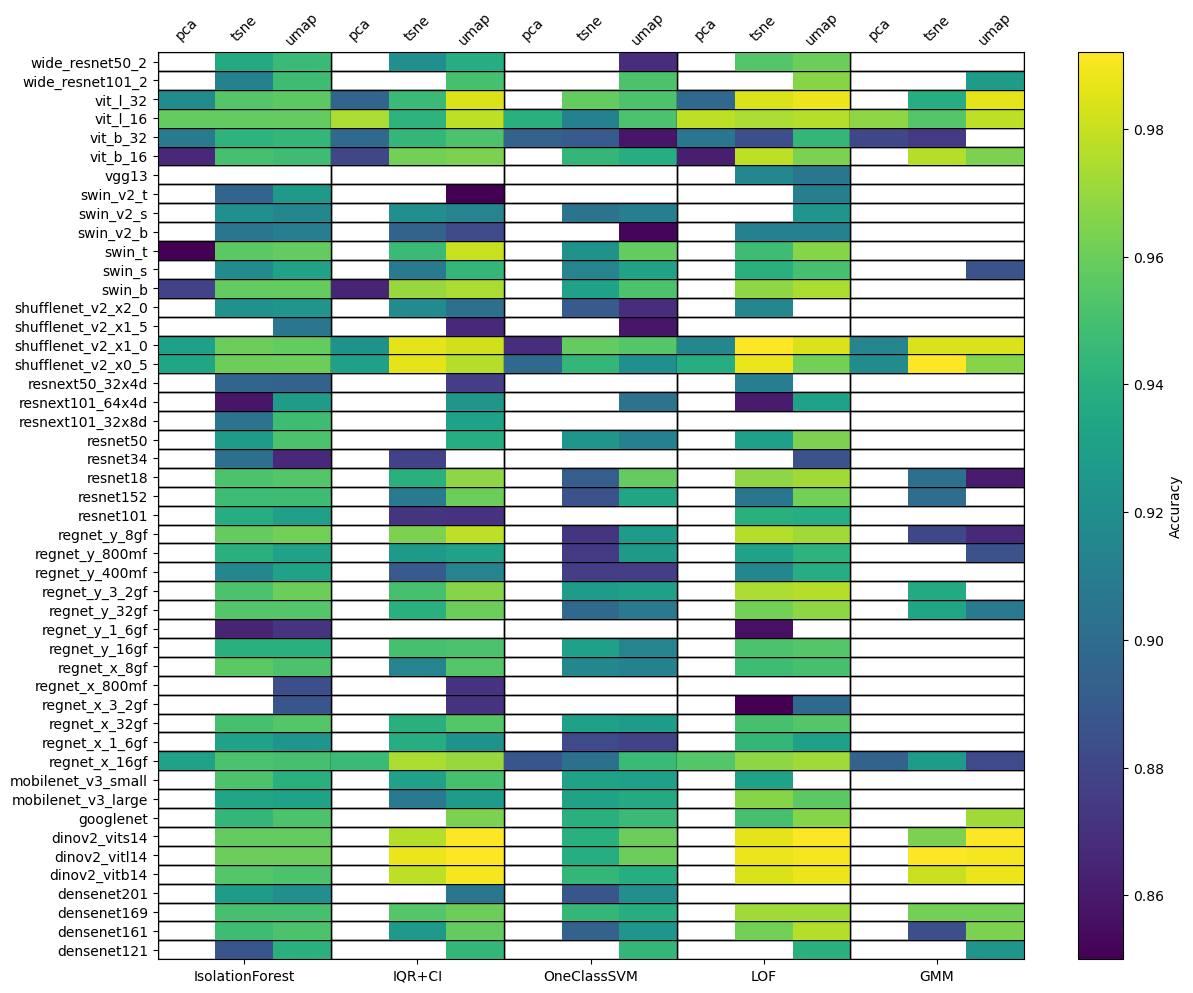
\includegraphics[width=17cm]{plots/anomaly_detection_plantvillage}
    \caption{Anomaly detection performance across different backbone architectures and dimensionality reduction techniques on the Plant Village dataset.
    Backbones on y-axis, anomaly detetection algorithm on lower x-axis, dimensionality reduction method on top x-axis.
    The color indicates the accuracy for each backbone-detection-reduction combination.}
    \label{fig:anomaly_detection_plantvillage}
\end{figure}

\begin{figure}[H]
    \centering
    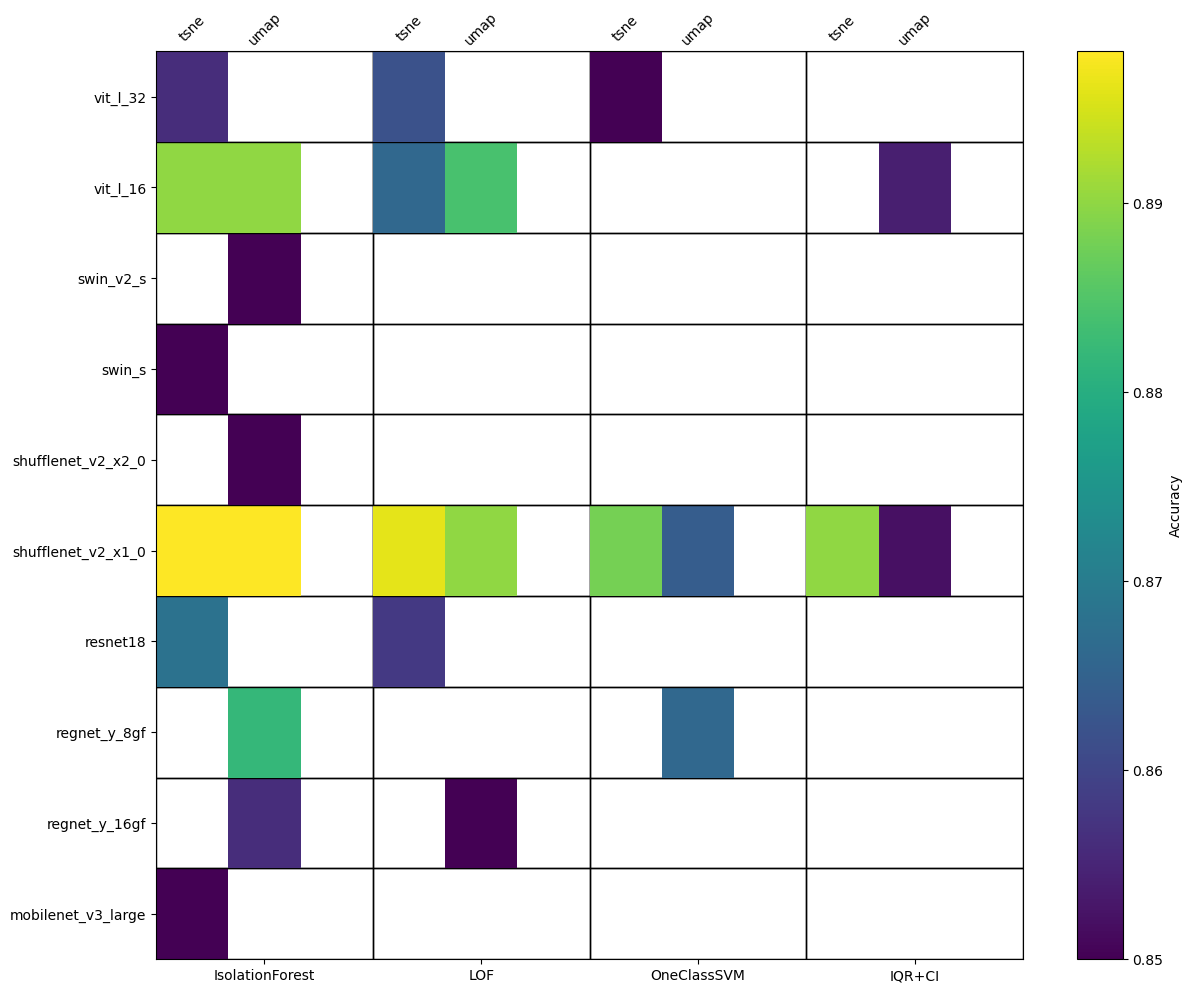
\includegraphics[width=17cm]{plots/anomaly_detection_plantpathology}
    \caption{Anomaly detection performance across different backbone architectures and dimensionality reduction techniques on the Plant Pathology dataset.
    Backbones on y-axis, anomaly detetection algorithm on lower x-axis, dimensionality reduction method on top x-axis.
    The color indicates the accuracy for each backbone-detection-reduction combination.}
    \label{fig:anomaly_detection_plantpathology}
\end{figure}

\begin{figure}[H]
    \centering
    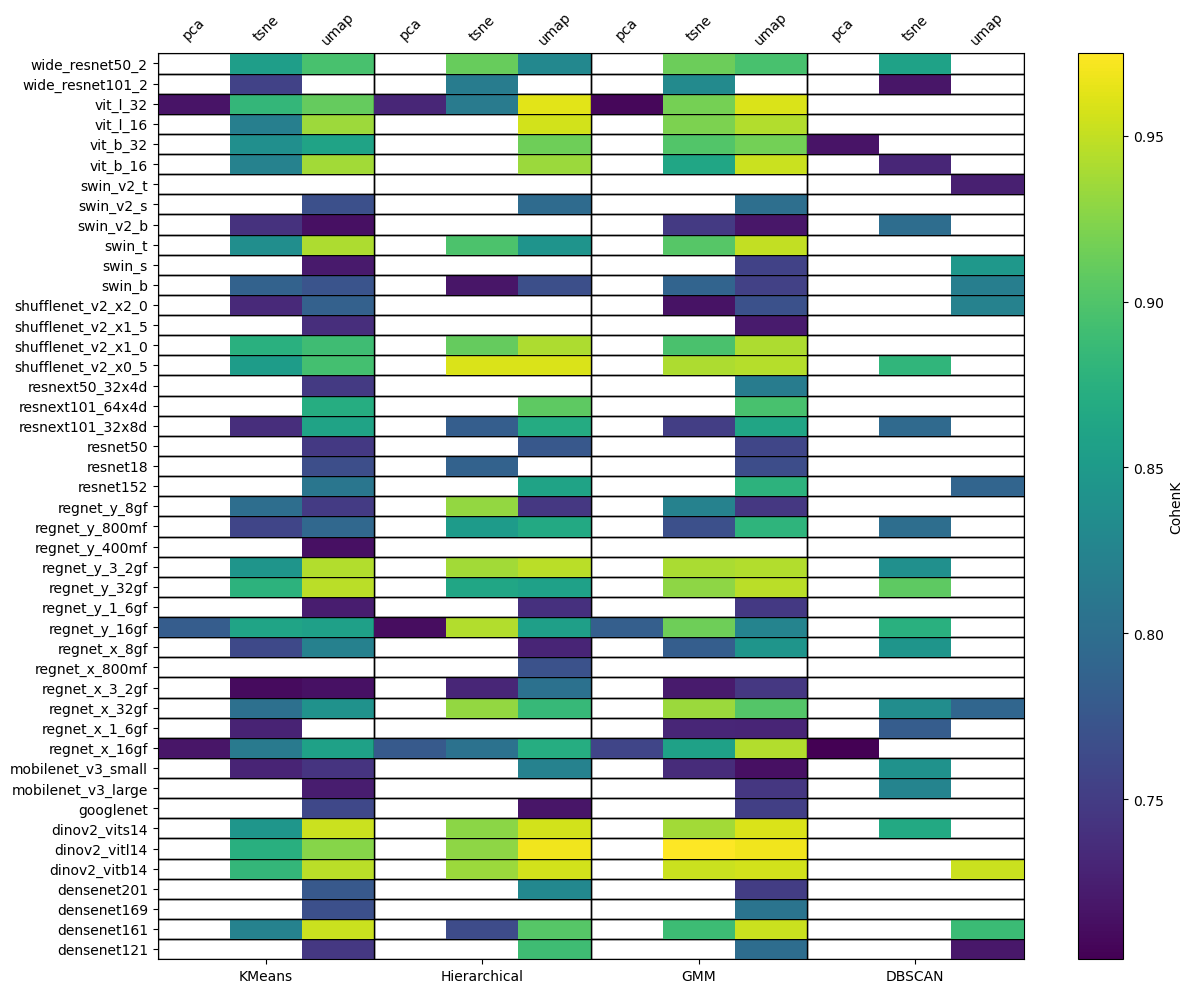
\includegraphics[width=17cm]{plots/clusterization_plantvillage}
    \caption{Clustering performance across different backbone architectures and dimensionality reduction techniques on the Plant Village dataset.
    Backbones on y-axis, clustering algorithm on lower x-axis, dimensionality reduction method on top x-axis.
    The color indicates the accuracy for each backbone-detection-reduction combination.}
    \label{fig:clusterization_plantvillage}
\end{figure}

\begin{figure}[H]
    \centering
    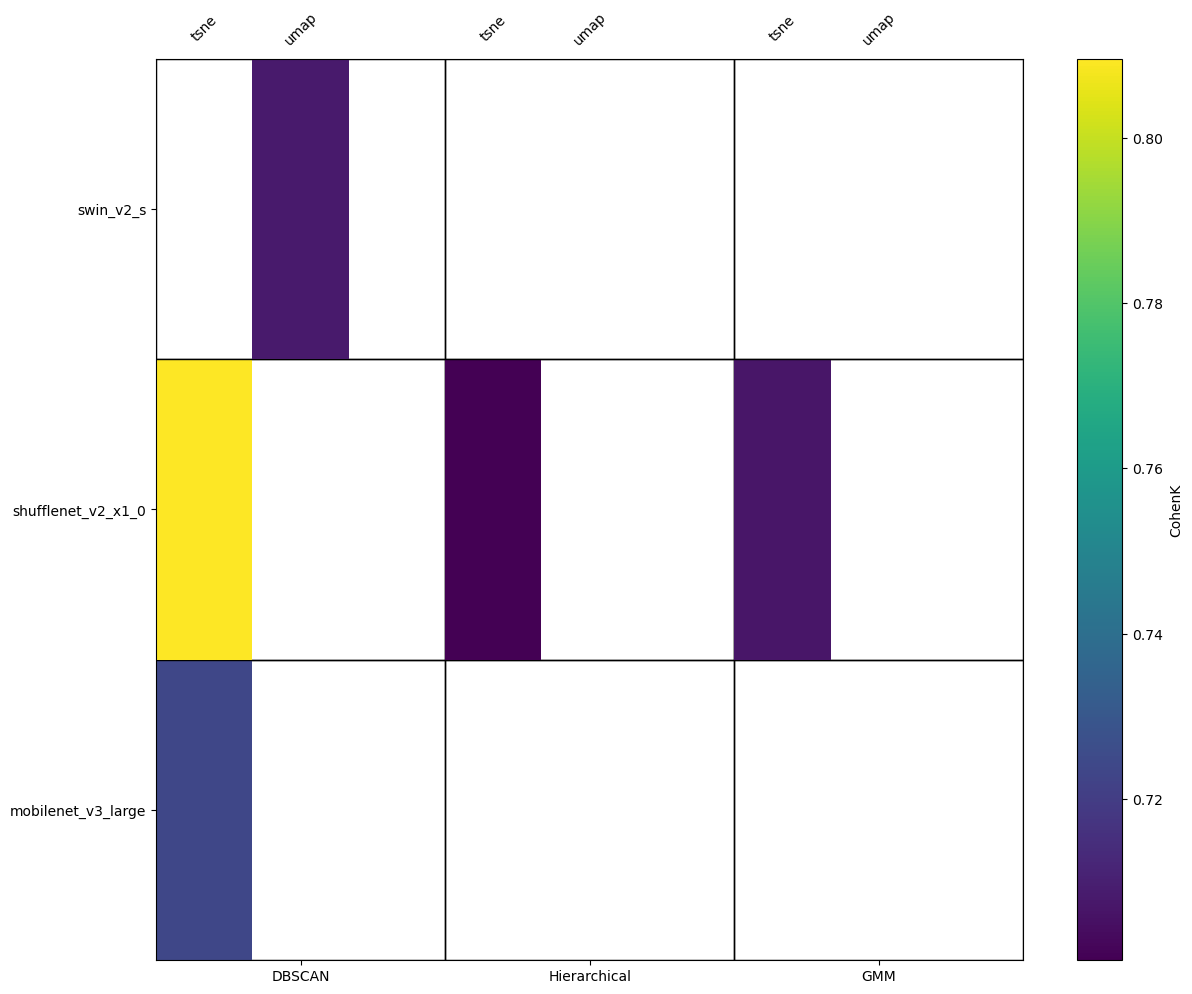
\includegraphics[width=17cm]{plots/clusterization_plantpathology}
    \caption{Clustering performance across different backbone architectures and dimensionality reduction techniques on the Plant Pathology dataset.
    Backbones on y-axis, clustering algorithm on lower x-axis, dimensionality reduction method on top x-axis.
    The color indicates the accuracy for each backbone-detection-reduction combination.}
    \label{fig:clusterization_plantpathology}
\end{figure}

\textbf{Dataset related performances}

The analysis of performance metrics across datasets revealed significant differences 
in model efficacy between laboratory-acquired and field-acquired images. 
The Plant Village dataset, consisting of controlled laboratory images with segmented 
leaves against uniform backgrounds, consistently enabled superior performance compared 
to the Plant Pathology dataset across all evaluation metrics.

For anomaly detection tasks, accuracy scores on the Plant Village dataset frequently 
exceeded 90\%, as shown in Figure~\ref{fig:anomaly_detection_plantvillage}. In contrast, 
the same architectures applied to the Plant Pathology dataset did not achieved
the benchmark or got a performance decrease of approximately 
5-10\%, as illustrated in Figure~\ref{fig:anomaly_detection_plantpathology}.

This performance gap was even more pronounced in clustering tasks, where Cohen's Kappa 
coefficients reached as high as 0.9 with 12 backbones on Plant Village data but 
peaked at 0.80 on 
Plant Pathology data and achived benchmark with only three backbones, 
as seen in Figures~\ref{fig:clusterization_plantvillage} and 
\ref{fig:clusterization_plantpathology}. The controlled environment and object-focused 
nature of the Plant Village dataset allowed models to concentrate on leaf 
characteristics directly relevant to disease detection without the confounding 
variables present in field conditions.

The Plant Pathology dataset's variable lighting, complex backgrounds, and inconsistent 
perspectives presented a substantially more challenging scenario for feature extraction
focusing on diseseas sympthoms.

These findings highlight the significant challenge of transitioning plant disease 
detection systems from controlled laboratory environments to real-world field 
applications, where background elements and environmental variability introduce 
substantial complexity to the feature extraction and classification process.

Nethertheless, the benchmark was achieved also for the challenging field-acquired
images, indicating that the selected architectures and methods are capable of
generalizing to real-world conditions.

\textbf{Effect of Feature Extraction Architecture}

Among the tested architectures, the ShuffleNet\_v2 feature extractor consistently demonstrated strong 
performance across both datasets, with the x1\_0 size version achieving 
the benchmark for both anomaly and clusterization tasks.
Other well performing architectures
were DINOv2 and ViT on Plant Village dataset for both tasks, but they did not 
perform consistently on the Plant Pathology dataset.
Remarkably ShuffleNet\_v2\_x1\_0 is a lightweight architecture with only 2.3M parameters,
in respect to the DINOv2 and ViT architectures which have 300M and 86M parameters respectively.
This suggests that the selected feature extractors are capable of achieving high performance
even with limited computational resources, making them suitable for deployment in
resource-constrained environments. 

\textbf{Impact of Dimensionality Reduction}

Different dimensionality reduction techniques showed varying effectiveness:

\begin{itemize}
    \item \textbf{t-SNE} consistently yielded the highest performances on both tasks and datasets when in combination with ShuffleNet\_v2\_x1\_0.
    \item \textbf{UMAP} performed competitively with t-SNE, in some cases surpassing it, but not the best option for all tasks and datasets.
    \item \textbf{PCA}, while computationally efficient, generally produced lower accuracy compared to t-SNE and UMAP, indicating that linear dimensionality reduction may not sufficiently preserve the complex structure necessary for plant disease detection.
\end{itemize}

The choice of dimensionality reduction technique significantly influenced the performance of both anomaly detection and clustering tasks. t-SNE and UMAP were particularly effective in preserving the local structure of the data, leading to better separability of classes in the reduced feature space.

\textbf{Comparison of Anomaly Detection Algorithms}

Among the tested anomaly detection algorithms:

\begin{itemize}
    \item \textbf{Isolation Forest} exalled on Plant Pathology dataset while the performances with Plant Village were low in respect to the others methods.
    \item \textbf{One-Class SVM} did not exalled on any of the datasets.
    \item \textbf{LOF} showed the most stable performances.
    \item \textbf{GMM} demonstrated comparable performance with LOF on Plant Village, but it never reached the benchmark on Plant Pathology.
    \item \textbf{IQR with Confidence Interval}, while simpler than the machine learning approaches, still achieved respectable performance on both datasets, highlighting the effectiveness of statistical approaches for this task.
\end{itemize}

The Plant Pathology dataset generally yielded lower performance compared to Plant Village across all algorithms, reflecting the greater difficulty of analyzing field-acquired images with variable conditions.

\textbf{Clustering Performance}

The clustering-based classification approach revealed complementary insights about the discriminative power of extracted features.

\begin{itemize}
    \item \textbf{K-Means, Hierarchical, and GMM} Good results on Plant Village achieving benchmark with multiple backbones, but on Plant Pathology only K-Means and GMM reached the benchmark.
    \item \textbf{DBSCAN} achieved the benchmark on Plant Village with less backbones in respect the other methods, while on Plant Pathology achieved the best result with ShuffleNet\_v2\_x1\_0.
\end{itemize}

The clustering-based classification approach revealed complementary insights about the discriminative power of extracted features, with significant differences in algorithm performance across datasets.

\begin{itemize}
    \item \textbf{K-Means, Hierarchical, and GMM} achieved strong results on Plant Village, reaching the benchmark with multiple backbone architectures. However, on the more challenging Plant Pathology dataset, only K-Means and GMM reached the benchmark. This suggests that centroid and distribution-based approaches perform consistently when the number of clusters is explicitly defined to match the disease classes.
    
    \item \textbf{DBSCAN} exhibited a distinct behavior pattern, achieving the benchmark on Plant Village with fewer backbones compared to other methods, while on Plant Pathology it achieved the best overall result specifically with ShuffleNet\_v2\_x1\_0. This unique performance profile can be attributed to DBSCAN's density-based approach, which differs fundamentally from the other algorithms in several ways:
    \begin{itemize}
        \item Unlike parametric methods that assume specific cluster shapes, DBSCAN identifies arbitrarily shaped clusters based on density variations, potentially capturing the complex symptom patterns in field conditions more effectively.
        
        \item DBSCAN automatically estimates its critical epsilon parameter based on the nearest neighbor distances in the feature space, making it particularly responsive to the actual distribution characteristics rather than prior assumptions.
        
        \item Its built-in outlier detection capability, which labels points in low-density regions as noise, provides natural robustness against the variable imaging conditions present in the Plant Pathology dataset.
        
        \item The exceptional performance with ShuffleNet\_v2\_x1\_0 suggests this lightweight architecture (2.3M parameters) produces feature distributions with clearer density gradients between disease classes, despite having significantly fewer parameters than transformer-based alternatives.
    \end{itemize}
\end{itemize}

These findings indicate that while conventional clustering methods perform well in controlled environments, density-based approaches may offer advantages for disease detection in variable field conditions, particularly when paired with efficient feature extractors that create well-separated density regions in the feature space.

\section{Conclusions}

This comprehensive evaluation of neural network architectures as feature extractors for plant disease anomaly detection has yielded several important findings with significant implications for agricultural monitoring applications.

Our first key finding revealed a consistent performance gap between laboratory and field-acquired images, with detection accuracy typically 5-10\% lower on field images. This quantifies the substantial challenge of translating plant disease detection systems from controlled environments to practical field applications. Despite this gap, our study identified combinations of feature extractors and detection algorithms that achieved benchmark performance even in challenging field conditions, demonstrating that robust field-deployable systems are achievable.

The ShuffleNet\_v2\_x1\_0 architecture emerged as the most consistently effective feature extractor across both datasets and evaluation methodologies. Remarkably, this lightweight network (2.3M parameters) outperformed substantially larger models like DINOv2 (300M parameters) and ViT (86M parameters) in field conditions. This finding challenges the common assumption that larger, more complex models necessarily yield better performance for specialized tasks. Instead, it suggests that computational efficiency and targeted feature extraction may be more valuable than model capacity for plant disease detection, particularly in resource-constrained deployment scenarios.

Among dimensionality reduction techniques, t-SNE consistently yielded the highest performance across most configurations, with UMAP following closely. The substantially lower performance of PCA indicates that nonlinear dimensionality reduction techniques better preserve the complex feature relationships crucial for disease differentiation. This finding highlights the importance of maintaining local neighborhood structures in the reduced feature space for effective anomaly detection.

The comparison of anomaly detection algorithms revealed that LOF demonstrated the most stable performance across datasets, while Isolation Forest excelled specifically on field-acquired images. This suggests that different detection methodologies have complementary strengths depending on image acquisition conditions. For practical field applications, ensemble approaches combining multiple detection algorithms might prove beneficial.

For clustering-based classification, DBSCAN with ShuffleNet\_v2\_x1\_0 achieved superior performance on field images compared to other combinations. This density-based approach appears particularly well-suited to handling the variable imaging conditions present in field settings, capturing the natural density variations between healthy and diseased samples in the feature space.

These findings have important practical implications for agricultural disease monitoring systems. By selecting lightweight, efficient architectures like ShuffleNet\_v2\_x1\_0, developers can create deployment-ready solutions for resource-constrained environments such as edge devices or mobile applications. The established benchmark performance on field-acquired images demonstrates that anomaly detection approaches are viable alternatives to supervised classification, especially in scenarios where obtaining comprehensive labeled datasets for every potential disease is impractical.

Future research directions should explore fine-tuning strategies specifically for agricultural domain adaptation, which may further close the performance gap between laboratory and field conditions. Additionally, investigating temporal anomaly detection for disease progression monitoring and extending the approach to multi-spectral or hyperspectral imagery could enhance detection capabilities, particularly for early-stage infections. Finally, developing integrated systems that combine anomaly detection with targeted classification for identified anomalies could create more comprehensive disease management solutions for practical agricultural applications.

In conclusion, this study establishes that computationally efficient feature extraction architectures, when combined with appropriate dimensionality reduction and anomaly detection algorithms, can effectively identify plant diseases across varying imaging conditions. These findings provide a foundation for developing practical, field-deployable systems for early disease detection that can contribute to sustainable agricultural practices and improved food security.

\bibliographystyle{plainnat}
\bibliography{Anomaly_detection}

\end{document}